% Created by tikzDevice version 0.12.6 on 2023-12-11 01:26:35
% !TEX encoding = UTF-8 Unicode
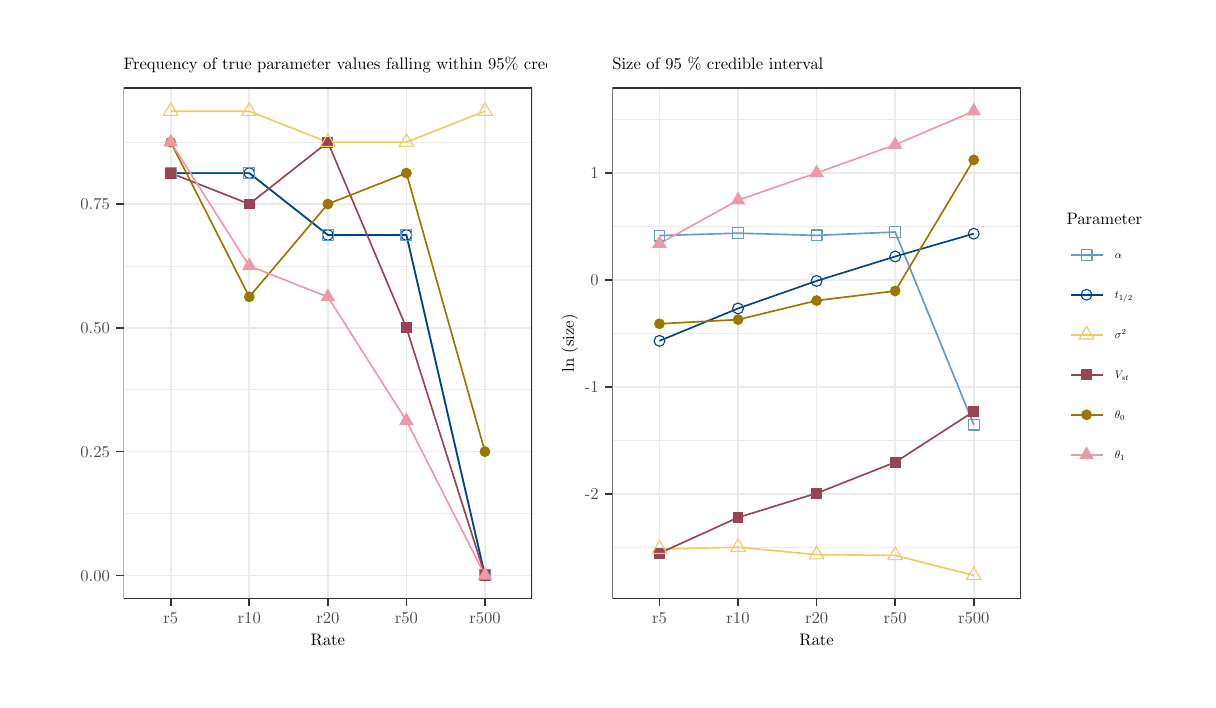
\begin{tikzpicture}[x=1pt,y=1pt]
\definecolor{fillColor}{RGB}{255,255,255}
\path[use as bounding box,fill=fillColor,fill opacity=0.00] (0,0) rectangle (419.17,235.60);
\begin{scope}
\path[clip] (  0.00,  0.00) rectangle (419.17,235.60);
\definecolor{drawColor}{RGB}{255,255,255}
\definecolor{fillColor}{RGB}{255,255,255}

\path[draw=drawColor,line width= 0.6pt,line join=round,line cap=round,fill=fillColor] (  0.00,  0.00) rectangle (419.17,235.60);
\end{scope}
\begin{scope}
\path[clip] (  5.50,  5.50) rectangle (187.78,230.10);
\definecolor{drawColor}{RGB}{255,255,255}
\definecolor{fillColor}{RGB}{255,255,255}

\path[draw=drawColor,line width= 0.6pt,line join=round,line cap=round,fill=fillColor] (  5.50,  5.50) rectangle (187.78,230.10);
\end{scope}
\begin{scope}
\path[clip] ( 34.66, 29.30) rectangle (182.28,213.80);
\definecolor{fillColor}{RGB}{255,255,255}

\path[fill=fillColor] ( 34.66, 29.30) rectangle (182.28,213.80);
\definecolor{drawColor}{gray}{0.92}

\path[draw=drawColor,line width= 0.3pt,line join=round] ( 34.66, 60.05) --
	(182.28, 60.05);

\path[draw=drawColor,line width= 0.3pt,line join=round] ( 34.66,104.78) --
	(182.28,104.78);

\path[draw=drawColor,line width= 0.3pt,line join=round] ( 34.66,149.50) --
	(182.28,149.50);

\path[draw=drawColor,line width= 0.3pt,line join=round] ( 34.66,194.23) --
	(182.28,194.23);

\path[draw=drawColor,line width= 0.6pt,line join=round] ( 34.66, 37.68) --
	(182.28, 37.68);

\path[draw=drawColor,line width= 0.6pt,line join=round] ( 34.66, 82.41) --
	(182.28, 82.41);

\path[draw=drawColor,line width= 0.6pt,line join=round] ( 34.66,127.14) --
	(182.28,127.14);

\path[draw=drawColor,line width= 0.6pt,line join=round] ( 34.66,171.87) --
	(182.28,171.87);

\path[draw=drawColor,line width= 0.6pt,line join=round] ( 51.70, 29.30) --
	( 51.70,213.80);

\path[draw=drawColor,line width= 0.6pt,line join=round] ( 80.08, 29.30) --
	( 80.08,213.80);

\path[draw=drawColor,line width= 0.6pt,line join=round] (108.47, 29.30) --
	(108.47,213.80);

\path[draw=drawColor,line width= 0.6pt,line join=round] (136.86, 29.30) --
	(136.86,213.80);

\path[draw=drawColor,line width= 0.6pt,line join=round] (165.24, 29.30) --
	(165.24,213.80);
\definecolor{drawColor}{RGB}{102,153,204}

\path[draw=drawColor,line width= 0.6pt,line join=round] ( 51.70,183.05) --
	( 80.08,183.05) --
	(108.47,160.69) --
	(136.86,160.69) --
	(165.24, 37.68);
\definecolor{drawColor}{RGB}{0,68,136}

\path[draw=drawColor,line width= 0.6pt,line join=round] ( 51.70,183.05) --
	( 80.08,183.05) --
	(108.47,160.69) --
	(136.86,160.69) --
	(165.24, 37.68);
\definecolor{drawColor}{RGB}{238,204,102}

\path[draw=drawColor,line width= 0.6pt,line join=round] ( 51.70,205.41) --
	( 80.08,205.41) --
	(108.47,194.23) --
	(136.86,194.23) --
	(165.24,205.41);
\definecolor{drawColor}{RGB}{153,68,85}

\path[draw=drawColor,line width= 0.6pt,line join=round] ( 51.70,183.05) --
	( 80.08,171.87) --
	(108.47,194.23) --
	(136.86,127.14) --
	(165.24, 37.68);
\definecolor{drawColor}{RGB}{153,119,0}

\path[draw=drawColor,line width= 0.6pt,line join=round] ( 51.70,194.23) --
	( 80.08,138.32) --
	(108.47,171.87) --
	(136.86,183.05) --
	(165.24, 82.41);
\definecolor{drawColor}{RGB}{238,153,170}

\path[draw=drawColor,line width= 0.6pt,line join=round] ( 51.70,194.23) --
	( 80.08,149.50) --
	(108.47,138.32) --
	(136.86, 93.59) --
	(165.24, 37.68);
\definecolor{drawColor}{RGB}{0,68,136}

\path[draw=drawColor,line width= 0.4pt,line join=round,line cap=round] ( 51.70,183.05) circle (  1.96);
\definecolor{drawColor}{RGB}{102,153,204}

\path[draw=drawColor,line width= 0.4pt,line join=round,line cap=round] ( 49.73,181.09) rectangle ( 53.66,185.01);
\definecolor{fillColor}{RGB}{153,68,85}

\path[fill=fillColor] ( 49.73,181.09) --
	( 53.66,181.09) --
	( 53.66,185.01) --
	( 49.73,185.01) --
	cycle;
\definecolor{drawColor}{RGB}{238,204,102}

\path[draw=drawColor,line width= 0.4pt,line join=round,line cap=round] ( 51.70,208.47) --
	( 54.34,203.89) --
	( 49.05,203.89) --
	cycle;
\definecolor{fillColor}{RGB}{153,119,0}

\path[fill=fillColor] ( 51.70,194.23) circle (  1.96);
\definecolor{fillColor}{RGB}{238,153,170}

\path[fill=fillColor] ( 51.70,197.28) --
	( 54.34,192.71) --
	( 49.05,192.71) --
	cycle;
\definecolor{drawColor}{RGB}{0,68,136}

\path[draw=drawColor,line width= 0.4pt,line join=round,line cap=round] ( 80.08,183.05) circle (  1.96);
\definecolor{drawColor}{RGB}{102,153,204}

\path[draw=drawColor,line width= 0.4pt,line join=round,line cap=round] ( 78.12,181.09) rectangle ( 82.04,185.01);
\definecolor{fillColor}{RGB}{153,68,85}

\path[fill=fillColor] ( 78.12,169.91) --
	( 82.04,169.91) --
	( 82.04,173.83) --
	( 78.12,173.83) --
	cycle;
\definecolor{drawColor}{RGB}{238,204,102}

\path[draw=drawColor,line width= 0.4pt,line join=round,line cap=round] ( 80.08,208.47) --
	( 82.73,203.89) --
	( 77.44,203.89) --
	cycle;
\definecolor{fillColor}{RGB}{153,119,0}

\path[fill=fillColor] ( 80.08,138.32) circle (  1.96);
\definecolor{fillColor}{RGB}{238,153,170}

\path[fill=fillColor] ( 80.08,152.56) --
	( 82.73,147.98) --
	( 77.44,147.98) --
	cycle;
\definecolor{drawColor}{RGB}{0,68,136}

\path[draw=drawColor,line width= 0.4pt,line join=round,line cap=round] (108.47,160.69) circle (  1.96);
\definecolor{drawColor}{RGB}{102,153,204}

\path[draw=drawColor,line width= 0.4pt,line join=round,line cap=round] (106.51,158.72) rectangle (110.43,162.65);
\definecolor{fillColor}{RGB}{153,68,85}

\path[fill=fillColor] (106.51,192.27) --
	(110.43,192.27) --
	(110.43,196.19) --
	(106.51,196.19) --
	cycle;
\definecolor{drawColor}{RGB}{238,204,102}

\path[draw=drawColor,line width= 0.4pt,line join=round,line cap=round] (108.47,197.28) --
	(111.11,192.71) --
	(105.83,192.71) --
	cycle;
\definecolor{fillColor}{RGB}{153,119,0}

\path[fill=fillColor] (108.47,171.87) circle (  1.96);
\definecolor{fillColor}{RGB}{238,153,170}

\path[fill=fillColor] (108.47,141.37) --
	(111.11,136.80) --
	(105.83,136.80) --
	cycle;
\definecolor{drawColor}{RGB}{0,68,136}

\path[draw=drawColor,line width= 0.4pt,line join=round,line cap=round] (136.86,160.69) circle (  1.96);
\definecolor{drawColor}{RGB}{102,153,204}

\path[draw=drawColor,line width= 0.4pt,line join=round,line cap=round] (134.90,158.72) rectangle (138.82,162.65);
\definecolor{fillColor}{RGB}{153,68,85}

\path[fill=fillColor] (134.90,125.18) --
	(138.82,125.18) --
	(138.82,129.10) --
	(134.90,129.10) --
	cycle;
\definecolor{drawColor}{RGB}{238,204,102}

\path[draw=drawColor,line width= 0.4pt,line join=round,line cap=round] (136.86,197.28) --
	(139.50,192.71) --
	(134.21,192.71) --
	cycle;
\definecolor{fillColor}{RGB}{153,119,0}

\path[fill=fillColor] (136.86,183.05) circle (  1.96);
\definecolor{fillColor}{RGB}{238,153,170}

\path[fill=fillColor] (136.86, 96.65) --
	(139.50, 92.07) --
	(134.21, 92.07) --
	cycle;
\definecolor{drawColor}{RGB}{0,68,136}

\path[draw=drawColor,line width= 0.4pt,line join=round,line cap=round] (165.24, 37.68) circle (  1.96);
\definecolor{drawColor}{RGB}{102,153,204}

\path[draw=drawColor,line width= 0.4pt,line join=round,line cap=round] (163.28, 35.72) rectangle (167.21, 39.65);
\definecolor{fillColor}{RGB}{153,68,85}

\path[fill=fillColor] (163.28, 35.72) --
	(167.21, 35.72) --
	(167.21, 39.65) --
	(163.28, 39.65) --
	cycle;
\definecolor{drawColor}{RGB}{238,204,102}

\path[draw=drawColor,line width= 0.4pt,line join=round,line cap=round] (165.24,208.47) --
	(167.89,203.89) --
	(162.60,203.89) --
	cycle;
\definecolor{fillColor}{RGB}{153,119,0}

\path[fill=fillColor] (165.24, 82.41) circle (  1.96);
\definecolor{fillColor}{RGB}{238,153,170}

\path[fill=fillColor] (165.24, 40.74) --
	(167.89, 36.16) --
	(162.60, 36.16) --
	cycle;
\definecolor{drawColor}{gray}{0.20}

\path[draw=drawColor,line width= 0.6pt,line join=round,line cap=round] ( 34.66, 29.30) rectangle (182.28,213.80);
\end{scope}
\begin{scope}
\path[clip] (  0.00,  0.00) rectangle (419.17,235.60);
\definecolor{drawColor}{gray}{0.30}

\node[text=drawColor,anchor=base east,inner sep=0pt, outer sep=0pt, scale=  0.60] at ( 29.71, 35.62) {0.00};

\node[text=drawColor,anchor=base east,inner sep=0pt, outer sep=0pt, scale=  0.60] at ( 29.71, 80.35) {0.25};

\node[text=drawColor,anchor=base east,inner sep=0pt, outer sep=0pt, scale=  0.60] at ( 29.71,125.07) {0.50};

\node[text=drawColor,anchor=base east,inner sep=0pt, outer sep=0pt, scale=  0.60] at ( 29.71,169.80) {0.75};
\end{scope}
\begin{scope}
\path[clip] (  0.00,  0.00) rectangle (419.17,235.60);
\definecolor{drawColor}{gray}{0.20}

\path[draw=drawColor,line width= 0.6pt,line join=round] ( 31.91, 37.68) --
	( 34.66, 37.68);

\path[draw=drawColor,line width= 0.6pt,line join=round] ( 31.91, 82.41) --
	( 34.66, 82.41);

\path[draw=drawColor,line width= 0.6pt,line join=round] ( 31.91,127.14) --
	( 34.66,127.14);

\path[draw=drawColor,line width= 0.6pt,line join=round] ( 31.91,171.87) --
	( 34.66,171.87);
\end{scope}
\begin{scope}
\path[clip] (  0.00,  0.00) rectangle (419.17,235.60);
\definecolor{drawColor}{gray}{0.20}

\path[draw=drawColor,line width= 0.6pt,line join=round] ( 51.70, 26.55) --
	( 51.70, 29.30);

\path[draw=drawColor,line width= 0.6pt,line join=round] ( 80.08, 26.55) --
	( 80.08, 29.30);

\path[draw=drawColor,line width= 0.6pt,line join=round] (108.47, 26.55) --
	(108.47, 29.30);

\path[draw=drawColor,line width= 0.6pt,line join=round] (136.86, 26.55) --
	(136.86, 29.30);

\path[draw=drawColor,line width= 0.6pt,line join=round] (165.24, 26.55) --
	(165.24, 29.30);
\end{scope}
\begin{scope}
\path[clip] (  0.00,  0.00) rectangle (419.17,235.60);
\definecolor{drawColor}{gray}{0.30}

\node[text=drawColor,anchor=base,inner sep=0pt, outer sep=0pt, scale=  0.60] at ( 51.70, 20.22) {r5};

\node[text=drawColor,anchor=base,inner sep=0pt, outer sep=0pt, scale=  0.60] at ( 80.08, 20.22) {r10};

\node[text=drawColor,anchor=base,inner sep=0pt, outer sep=0pt, scale=  0.60] at (108.47, 20.22) {r20};

\node[text=drawColor,anchor=base,inner sep=0pt, outer sep=0pt, scale=  0.60] at (136.86, 20.22) {r50};

\node[text=drawColor,anchor=base,inner sep=0pt, outer sep=0pt, scale=  0.60] at (165.24, 20.22) {r500};
\end{scope}
\begin{scope}
\path[clip] (  0.00,  0.00) rectangle (419.17,235.60);
\definecolor{drawColor}{RGB}{0,0,0}

\node[text=drawColor,anchor=base,inner sep=0pt, outer sep=0pt, scale=  0.60] at (108.47, 12.17) {Rate};
\end{scope}
\begin{scope}
\path[clip] (  0.00,  0.00) rectangle (419.17,235.60);
\definecolor{drawColor}{RGB}{0,0,0}

\node[text=drawColor,anchor=base west,inner sep=0pt, outer sep=0pt, scale=  0.60] at ( 34.66,220.47) {Frequency of true parameter values falling within  $\newline 95\%$ credible interval};
\end{scope}
\begin{scope}
\path[clip] (187.78,  5.50) rectangle (413.67,230.10);
\definecolor{drawColor}{RGB}{255,255,255}
\definecolor{fillColor}{RGB}{255,255,255}

\path[draw=drawColor,line width= 0.6pt,line join=round,line cap=round,fill=fillColor] (187.78,  5.50) rectangle (413.67,230.10);
\end{scope}
\begin{scope}
\path[clip] (211.27, 29.30) rectangle (358.89,213.80);
\definecolor{fillColor}{RGB}{255,255,255}

\path[fill=fillColor] (211.27, 29.30) rectangle (358.89,213.80);
\definecolor{drawColor}{gray}{0.92}

\path[draw=drawColor,line width= 0.3pt,line join=round] (211.27, 47.68) --
	(358.89, 47.68);

\path[draw=drawColor,line width= 0.3pt,line join=round] (211.27, 86.38) --
	(358.89, 86.38);

\path[draw=drawColor,line width= 0.3pt,line join=round] (211.27,125.08) --
	(358.89,125.08);

\path[draw=drawColor,line width= 0.3pt,line join=round] (211.27,163.78) --
	(358.89,163.78);

\path[draw=drawColor,line width= 0.3pt,line join=round] (211.27,202.49) --
	(358.89,202.49);

\path[draw=drawColor,line width= 0.6pt,line join=round] (211.27, 67.03) --
	(358.89, 67.03);

\path[draw=drawColor,line width= 0.6pt,line join=round] (211.27,105.73) --
	(358.89,105.73);

\path[draw=drawColor,line width= 0.6pt,line join=round] (211.27,144.43) --
	(358.89,144.43);

\path[draw=drawColor,line width= 0.6pt,line join=round] (211.27,183.14) --
	(358.89,183.14);

\path[draw=drawColor,line width= 0.6pt,line join=round] (228.31, 29.30) --
	(228.31,213.80);

\path[draw=drawColor,line width= 0.6pt,line join=round] (256.69, 29.30) --
	(256.69,213.80);

\path[draw=drawColor,line width= 0.6pt,line join=round] (285.08, 29.30) --
	(285.08,213.80);

\path[draw=drawColor,line width= 0.6pt,line join=round] (313.47, 29.30) --
	(313.47,213.80);

\path[draw=drawColor,line width= 0.6pt,line join=round] (341.86, 29.30) --
	(341.86,213.80);
\definecolor{drawColor}{RGB}{102,153,204}

\path[draw=drawColor,line width= 0.6pt,line join=round] (228.31,160.47) --
	(256.69,161.35) --
	(285.08,160.54) --
	(313.47,161.76) --
	(341.86, 92.17);
\definecolor{drawColor}{RGB}{0,68,136}

\path[draw=drawColor,line width= 0.6pt,line join=round] (228.31,122.43) --
	(256.69,134.13) --
	(285.08,144.08) --
	(313.47,152.91) --
	(341.86,161.16);
\definecolor{drawColor}{RGB}{238,204,102}

\path[draw=drawColor,line width= 0.6pt,line join=round] (228.31, 47.18) --
	(256.69, 47.86) --
	(285.08, 45.18) --
	(313.47, 44.91) --
	(341.86, 37.68);
\definecolor{drawColor}{RGB}{153,68,85}

\path[draw=drawColor,line width= 0.6pt,line join=round] (228.31, 45.71) --
	(256.69, 58.59) --
	(285.08, 67.36) --
	(313.47, 78.56) --
	(341.86, 96.91);
\definecolor{drawColor}{RGB}{153,119,0}

\path[draw=drawColor,line width= 0.6pt,line join=round] (228.31,128.60) --
	(256.69,130.10) --
	(285.08,136.98) --
	(313.47,140.44) --
	(341.86,187.84);
\definecolor{drawColor}{RGB}{238,153,170}

\path[draw=drawColor,line width= 0.6pt,line join=round] (228.31,157.56) --
	(256.69,173.28) --
	(285.08,183.09) --
	(313.47,193.29) --
	(341.86,205.41);
\definecolor{drawColor}{RGB}{0,68,136}

\path[draw=drawColor,line width= 0.4pt,line join=round,line cap=round] (228.31,122.43) circle (  1.96);
\definecolor{drawColor}{RGB}{102,153,204}

\path[draw=drawColor,line width= 0.4pt,line join=round,line cap=round] (226.35,158.51) rectangle (230.27,162.43);
\definecolor{fillColor}{RGB}{153,68,85}

\path[fill=fillColor] (226.35, 43.75) --
	(230.27, 43.75) --
	(230.27, 47.68) --
	(226.35, 47.68) --
	cycle;
\definecolor{drawColor}{RGB}{238,204,102}

\path[draw=drawColor,line width= 0.4pt,line join=round,line cap=round] (228.31, 50.23) --
	(230.95, 45.65) --
	(225.66, 45.65) --
	cycle;
\definecolor{fillColor}{RGB}{153,119,0}

\path[fill=fillColor] (228.31,128.60) circle (  1.96);
\definecolor{fillColor}{RGB}{238,153,170}

\path[fill=fillColor] (228.31,160.61) --
	(230.95,156.03) --
	(225.66,156.03) --
	cycle;
\definecolor{drawColor}{RGB}{0,68,136}

\path[draw=drawColor,line width= 0.4pt,line join=round,line cap=round] (256.69,134.13) circle (  1.96);
\definecolor{drawColor}{RGB}{102,153,204}

\path[draw=drawColor,line width= 0.4pt,line join=round,line cap=round] (254.73,159.39) rectangle (258.66,163.31);
\definecolor{fillColor}{RGB}{153,68,85}

\path[fill=fillColor] (254.73, 56.63) --
	(258.66, 56.63) --
	(258.66, 60.56) --
	(254.73, 60.56) --
	cycle;
\definecolor{drawColor}{RGB}{238,204,102}

\path[draw=drawColor,line width= 0.4pt,line join=round,line cap=round] (256.69, 50.91) --
	(259.34, 46.33) --
	(254.05, 46.33) --
	cycle;
\definecolor{fillColor}{RGB}{153,119,0}

\path[fill=fillColor] (256.69,130.10) circle (  1.96);
\definecolor{fillColor}{RGB}{238,153,170}

\path[fill=fillColor] (256.69,176.33) --
	(259.34,171.75) --
	(254.05,171.75) --
	cycle;
\definecolor{drawColor}{RGB}{0,68,136}

\path[draw=drawColor,line width= 0.4pt,line join=round,line cap=round] (285.08,144.08) circle (  1.96);
\definecolor{drawColor}{RGB}{102,153,204}

\path[draw=drawColor,line width= 0.4pt,line join=round,line cap=round] (283.12,158.58) rectangle (287.04,162.50);
\definecolor{fillColor}{RGB}{153,68,85}

\path[fill=fillColor] (283.12, 65.40) --
	(287.04, 65.40) --
	(287.04, 69.33) --
	(283.12, 69.33) --
	cycle;
\definecolor{drawColor}{RGB}{238,204,102}

\path[draw=drawColor,line width= 0.4pt,line join=round,line cap=round] (285.08, 48.23) --
	(287.72, 43.65) --
	(282.44, 43.65) --
	cycle;
\definecolor{fillColor}{RGB}{153,119,0}

\path[fill=fillColor] (285.08,136.98) circle (  1.96);
\definecolor{fillColor}{RGB}{238,153,170}

\path[fill=fillColor] (285.08,186.15) --
	(287.72,181.57) --
	(282.44,181.57) --
	cycle;
\definecolor{drawColor}{RGB}{0,68,136}

\path[draw=drawColor,line width= 0.4pt,line join=round,line cap=round] (313.47,152.91) circle (  1.96);
\definecolor{drawColor}{RGB}{102,153,204}

\path[draw=drawColor,line width= 0.4pt,line join=round,line cap=round] (311.51,159.80) rectangle (315.43,163.73);
\definecolor{fillColor}{RGB}{153,68,85}

\path[fill=fillColor] (311.51, 76.59) --
	(315.43, 76.59) --
	(315.43, 80.52) --
	(311.51, 80.52) --
	cycle;
\definecolor{drawColor}{RGB}{238,204,102}

\path[draw=drawColor,line width= 0.4pt,line join=round,line cap=round] (313.47, 47.96) --
	(316.11, 43.39) --
	(310.83, 43.39) --
	cycle;
\definecolor{fillColor}{RGB}{153,119,0}

\path[fill=fillColor] (313.47,140.44) circle (  1.96);
\definecolor{fillColor}{RGB}{238,153,170}

\path[fill=fillColor] (313.47,196.34) --
	(316.11,191.76) --
	(310.83,191.76) --
	cycle;
\definecolor{drawColor}{RGB}{0,68,136}

\path[draw=drawColor,line width= 0.4pt,line join=round,line cap=round] (341.86,161.16) circle (  1.96);
\definecolor{drawColor}{RGB}{102,153,204}

\path[draw=drawColor,line width= 0.4pt,line join=round,line cap=round] (339.89, 90.20) rectangle (343.82, 94.13);
\definecolor{fillColor}{RGB}{153,68,85}

\path[fill=fillColor] (339.89, 94.95) --
	(343.82, 94.95) --
	(343.82, 98.87) --
	(339.89, 98.87) --
	cycle;
\definecolor{drawColor}{RGB}{238,204,102}

\path[draw=drawColor,line width= 0.4pt,line join=round,line cap=round] (341.86, 40.74) --
	(344.50, 36.16) --
	(339.21, 36.16) --
	cycle;
\definecolor{fillColor}{RGB}{153,119,0}

\path[fill=fillColor] (341.86,187.84) circle (  1.96);
\definecolor{fillColor}{RGB}{238,153,170}

\path[fill=fillColor] (341.86,208.47) --
	(344.50,203.89) --
	(339.21,203.89) --
	cycle;
\definecolor{drawColor}{gray}{0.20}

\path[draw=drawColor,line width= 0.6pt,line join=round,line cap=round] (211.27, 29.30) rectangle (358.89,213.80);
\end{scope}
\begin{scope}
\path[clip] (  0.00,  0.00) rectangle (419.17,235.60);
\definecolor{drawColor}{gray}{0.30}

\node[text=drawColor,anchor=base east,inner sep=0pt, outer sep=0pt, scale=  0.60] at (206.32, 64.97) {-2};

\node[text=drawColor,anchor=base east,inner sep=0pt, outer sep=0pt, scale=  0.60] at (206.32,103.67) {-1};

\node[text=drawColor,anchor=base east,inner sep=0pt, outer sep=0pt, scale=  0.60] at (206.32,142.37) {0};

\node[text=drawColor,anchor=base east,inner sep=0pt, outer sep=0pt, scale=  0.60] at (206.32,181.07) {1};
\end{scope}
\begin{scope}
\path[clip] (  0.00,  0.00) rectangle (419.17,235.60);
\definecolor{drawColor}{gray}{0.20}

\path[draw=drawColor,line width= 0.6pt,line join=round] (208.52, 67.03) --
	(211.27, 67.03);

\path[draw=drawColor,line width= 0.6pt,line join=round] (208.52,105.73) --
	(211.27,105.73);

\path[draw=drawColor,line width= 0.6pt,line join=round] (208.52,144.43) --
	(211.27,144.43);

\path[draw=drawColor,line width= 0.6pt,line join=round] (208.52,183.14) --
	(211.27,183.14);
\end{scope}
\begin{scope}
\path[clip] (  0.00,  0.00) rectangle (419.17,235.60);
\definecolor{drawColor}{gray}{0.20}

\path[draw=drawColor,line width= 0.6pt,line join=round] (228.31, 26.55) --
	(228.31, 29.30);

\path[draw=drawColor,line width= 0.6pt,line join=round] (256.69, 26.55) --
	(256.69, 29.30);

\path[draw=drawColor,line width= 0.6pt,line join=round] (285.08, 26.55) --
	(285.08, 29.30);

\path[draw=drawColor,line width= 0.6pt,line join=round] (313.47, 26.55) --
	(313.47, 29.30);

\path[draw=drawColor,line width= 0.6pt,line join=round] (341.86, 26.55) --
	(341.86, 29.30);
\end{scope}
\begin{scope}
\path[clip] (  0.00,  0.00) rectangle (419.17,235.60);
\definecolor{drawColor}{gray}{0.30}

\node[text=drawColor,anchor=base,inner sep=0pt, outer sep=0pt, scale=  0.60] at (228.31, 20.22) {r5};

\node[text=drawColor,anchor=base,inner sep=0pt, outer sep=0pt, scale=  0.60] at (256.69, 20.22) {r10};

\node[text=drawColor,anchor=base,inner sep=0pt, outer sep=0pt, scale=  0.60] at (285.08, 20.22) {r20};

\node[text=drawColor,anchor=base,inner sep=0pt, outer sep=0pt, scale=  0.60] at (313.47, 20.22) {r50};

\node[text=drawColor,anchor=base,inner sep=0pt, outer sep=0pt, scale=  0.60] at (341.86, 20.22) {r500};
\end{scope}
\begin{scope}
\path[clip] (  0.00,  0.00) rectangle (419.17,235.60);
\definecolor{drawColor}{RGB}{0,0,0}

\node[text=drawColor,anchor=base,inner sep=0pt, outer sep=0pt, scale=  0.60] at (285.08, 12.17) {Rate};
\end{scope}
\begin{scope}
\path[clip] (  0.00,  0.00) rectangle (419.17,235.60);
\definecolor{drawColor}{RGB}{0,0,0}

\node[text=drawColor,rotate= 90.00,anchor=base,inner sep=0pt, outer sep=0pt, scale=  0.60] at (197.41,121.55) {$\ln$ (size)};
\end{scope}
\begin{scope}
\path[clip] (  0.00,  0.00) rectangle (419.17,235.60);
\definecolor{fillColor}{RGB}{255,255,255}

\path[fill=fillColor] (369.89, 68.54) rectangle (408.17,174.56);
\end{scope}
\begin{scope}
\path[clip] (  0.00,  0.00) rectangle (419.17,235.60);
\definecolor{drawColor}{RGB}{0,0,0}

\node[text=drawColor,anchor=base west,inner sep=0pt, outer sep=0pt, scale=  0.60] at (375.39,164.35) {Parameter};
\end{scope}
\begin{scope}
\path[clip] (  0.00,  0.00) rectangle (419.17,235.60);
\definecolor{fillColor}{RGB}{255,255,255}

\path[fill=fillColor] (375.39,146.31) rectangle (389.84,160.76);
\end{scope}
\begin{scope}
\path[clip] (  0.00,  0.00) rectangle (419.17,235.60);
\definecolor{drawColor}{RGB}{102,153,204}

\path[draw=drawColor,line width= 0.6pt,line join=round] (376.83,153.54) -- (388.40,153.54);
\end{scope}
\begin{scope}
\path[clip] (  0.00,  0.00) rectangle (419.17,235.60);
\definecolor{drawColor}{RGB}{102,153,204}

\path[draw=drawColor,line width= 0.4pt,line join=round,line cap=round] (380.65,151.57) rectangle (384.58,155.50);
\end{scope}
\begin{scope}
\path[clip] (  0.00,  0.00) rectangle (419.17,235.60);
\definecolor{fillColor}{RGB}{255,255,255}

\path[fill=fillColor] (375.39,131.85) rectangle (389.84,146.31);
\end{scope}
\begin{scope}
\path[clip] (  0.00,  0.00) rectangle (419.17,235.60);
\definecolor{drawColor}{RGB}{0,68,136}

\path[draw=drawColor,line width= 0.6pt,line join=round] (376.83,139.08) -- (388.40,139.08);
\end{scope}
\begin{scope}
\path[clip] (  0.00,  0.00) rectangle (419.17,235.60);
\definecolor{drawColor}{RGB}{0,68,136}

\path[draw=drawColor,line width= 0.4pt,line join=round,line cap=round] (382.62,139.08) circle (  1.96);
\end{scope}
\begin{scope}
\path[clip] (  0.00,  0.00) rectangle (419.17,235.60);
\definecolor{fillColor}{RGB}{255,255,255}

\path[fill=fillColor] (375.39,117.40) rectangle (389.84,131.85);
\end{scope}
\begin{scope}
\path[clip] (  0.00,  0.00) rectangle (419.17,235.60);
\definecolor{drawColor}{RGB}{238,204,102}

\path[draw=drawColor,line width= 0.6pt,line join=round] (376.83,124.63) -- (388.40,124.63);
\end{scope}
\begin{scope}
\path[clip] (  0.00,  0.00) rectangle (419.17,235.60);
\definecolor{drawColor}{RGB}{238,204,102}

\path[draw=drawColor,line width= 0.4pt,line join=round,line cap=round] (382.62,127.68) --
	(385.26,123.10) --
	(379.97,123.10) --
	cycle;
\end{scope}
\begin{scope}
\path[clip] (  0.00,  0.00) rectangle (419.17,235.60);
\definecolor{fillColor}{RGB}{255,255,255}

\path[fill=fillColor] (375.39,102.95) rectangle (389.84,117.40);
\end{scope}
\begin{scope}
\path[clip] (  0.00,  0.00) rectangle (419.17,235.60);
\definecolor{drawColor}{RGB}{153,68,85}

\path[draw=drawColor,line width= 0.6pt,line join=round] (376.83,110.17) -- (388.40,110.17);
\end{scope}
\begin{scope}
\path[clip] (  0.00,  0.00) rectangle (419.17,235.60);
\definecolor{fillColor}{RGB}{153,68,85}

\path[fill=fillColor] (380.65,108.21) --
	(384.58,108.21) --
	(384.58,112.14) --
	(380.65,112.14) --
	cycle;
\end{scope}
\begin{scope}
\path[clip] (  0.00,  0.00) rectangle (419.17,235.60);
\definecolor{fillColor}{RGB}{255,255,255}

\path[fill=fillColor] (375.39, 88.49) rectangle (389.84,102.95);
\end{scope}
\begin{scope}
\path[clip] (  0.00,  0.00) rectangle (419.17,235.60);
\definecolor{drawColor}{RGB}{153,119,0}

\path[draw=drawColor,line width= 0.6pt,line join=round] (376.83, 95.72) -- (388.40, 95.72);
\end{scope}
\begin{scope}
\path[clip] (  0.00,  0.00) rectangle (419.17,235.60);
\definecolor{fillColor}{RGB}{153,119,0}

\path[fill=fillColor] (382.62, 95.72) circle (  1.96);
\end{scope}
\begin{scope}
\path[clip] (  0.00,  0.00) rectangle (419.17,235.60);
\definecolor{fillColor}{RGB}{255,255,255}

\path[fill=fillColor] (375.39, 74.04) rectangle (389.84, 88.49);
\end{scope}
\begin{scope}
\path[clip] (  0.00,  0.00) rectangle (419.17,235.60);
\definecolor{drawColor}{RGB}{238,153,170}

\path[draw=drawColor,line width= 0.6pt,line join=round] (376.83, 81.27) -- (388.40, 81.27);
\end{scope}
\begin{scope}
\path[clip] (  0.00,  0.00) rectangle (419.17,235.60);
\definecolor{fillColor}{RGB}{238,153,170}

\path[fill=fillColor] (382.62, 84.32) --
	(385.26, 79.74) --
	(379.97, 79.74) --
	cycle;
\end{scope}
\begin{scope}
\path[clip] (  0.00,  0.00) rectangle (419.17,235.60);
\definecolor{drawColor}{RGB}{0,0,0}

\node[text=drawColor,anchor=base west,inner sep=0pt, outer sep=0pt, scale=  0.40] at (392.84,152.16) {$\alpha$};
\end{scope}
\begin{scope}
\path[clip] (  0.00,  0.00) rectangle (419.17,235.60);
\definecolor{drawColor}{RGB}{0,0,0}

\node[text=drawColor,anchor=base west,inner sep=0pt, outer sep=0pt, scale=  0.40] at (392.84,137.70) {$t_{1/2}$};
\end{scope}
\begin{scope}
\path[clip] (  0.00,  0.00) rectangle (419.17,235.60);
\definecolor{drawColor}{RGB}{0,0,0}

\node[text=drawColor,anchor=base west,inner sep=0pt, outer sep=0pt, scale=  0.40] at (392.84,123.25) {$\sigma^2$};
\end{scope}
\begin{scope}
\path[clip] (  0.00,  0.00) rectangle (419.17,235.60);
\definecolor{drawColor}{RGB}{0,0,0}

\node[text=drawColor,anchor=base west,inner sep=0pt, outer sep=0pt, scale=  0.40] at (392.84,108.80) {$V_{st}$};
\end{scope}
\begin{scope}
\path[clip] (  0.00,  0.00) rectangle (419.17,235.60);
\definecolor{drawColor}{RGB}{0,0,0}

\node[text=drawColor,anchor=base west,inner sep=0pt, outer sep=0pt, scale=  0.40] at (392.84, 94.34) {$\theta_0$};
\end{scope}
\begin{scope}
\path[clip] (  0.00,  0.00) rectangle (419.17,235.60);
\definecolor{drawColor}{RGB}{0,0,0}

\node[text=drawColor,anchor=base west,inner sep=0pt, outer sep=0pt, scale=  0.40] at (392.84, 79.89) {$\theta_1$};
\end{scope}
\begin{scope}
\path[clip] (  0.00,  0.00) rectangle (419.17,235.60);
\definecolor{drawColor}{RGB}{0,0,0}

\node[text=drawColor,anchor=base west,inner sep=0pt, outer sep=0pt, scale=  0.60] at (211.27,220.47) {Size of 95 $\%$ credible interval};
\end{scope}
\end{tikzpicture}
